\chapter{Stream Ciphers}\label{chap:streamcipher}
Sono una categoria di cifratori, tipicamente veloci nell'elaborazione del testo. Un esempio di stream cipher è il \textit{Vernam Cipher}. L'idea di base per uno stream cipher è quella di utilizzare una \textbf{chiave statica} che, unita ad un vettore di bit, permette di ottenere un messaggio cifrato.
\begin{figure}[h]
    \centering
    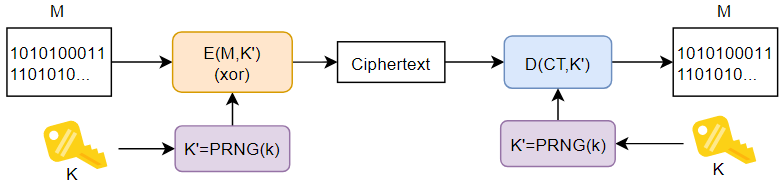
\includegraphics[width=\textwidth]{image/streamcipher.png}
    \caption{Stream Ciphers Scheme}
    \label{fig:stream_ciphers}
\end{figure}\\
In modo tale da rendere uno stream cipher sicuro da un \textit{CPA}, introduciamo il concetto di \textbf{Keystream}. Poiché una caratteristica richiesta per i cifratori era, la necessità di avere una chiave della stessa lunghezza del messaggio che fosse \textit{\textbf{sempre}} nuova, possiamo usare la chiave segreta precedentemente scambiata in qualche modo, come seed per un keystream generato tramite un algoritmo \textit{pseudorandom} che va in $xor$ con il messaggio.\\
\begin{remark}
E' importante non confondere la chiave random del One Time Pad con il keystream generato tramite algoritmo pseudorandom.
\end{remark}
\begin{remark}
L'algoritmo che genera il keystream è ciò che differenzia un cifratore dall'altro. Alcuni esempi sono \textbf{RC4, Salsa20, ChaCha20}.
\end{remark}
\begin{proposition}[Pro e Contro]
\begin{itemize}
    \item [\textcolor{green}{\textbf{PRO:}}]Lo schema in \cref{fig:stream_ciphers} permette di ottenere un testo cifrato in cui se una sotto-sequenza di bit si ripete, ogniuna verrà cifrata \textbf{sempre} in modo diverso.
    \item [\textcolor{red}{\textbf{CONS:}}]Se il messaggio viene cifrato una seconda volta, il testo cifrato sarà comunque \textbf{sempre} uguale a se stesso.
\end{itemize}
\end{proposition}
\section{Gli Initialization Vectors}
Poiché uno stream cipher implica l'utilizzo di una chiave statica e l'algoritmo di pseudo-random è deterministo per definizione, un messaggio verrà cifrato sempre nello stesso modo. Questo significa che perdiamo la proprietà di \textit{IND-CPA}.\\
Gli Initialization Vectors sono dei vettori di numeri generati randomicamente ad ogni nuovo messaggio inviato che permettono di mantenere una \textit{sicurezza semantica}\footnotemark  a patto che \textbf{\textit{non si ripetano MAI}}.
\footnotetext{Un cifratore è \textbf{semantically secure} se è impossibile estrarre informazioni sensibili del plain-text dal cipher-text.}
\begin{figure}[ht]
    \centering
    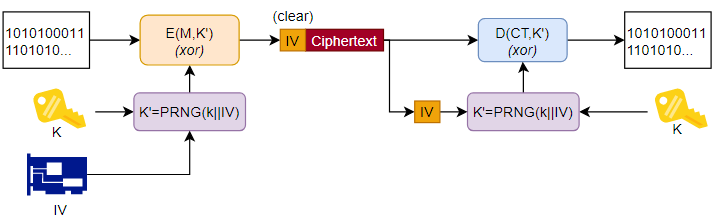
\includegraphics[width=\textwidth]{image/streamIV.png}
    \caption{Stream Ciphers with IV}
    \label{fig:streamiv}
\end{figure}\\
Abbiamo diversi modi per generare degli IV che siano sempre nuovi, al fine di applicare lo schema in \cref{fig:streamiv}:

\begin{itemize}
    \item \textbf{(Truly) Random:} ovvio. Di positivo ha che non può essere predibile, ma non realizzabile se non affidandosi ad effettive fluttuazioni naturali.
    \item \textbf{Sequence Number:} un numero di sequenza può essere sempre nuovo, ma può essere predetto, ad esempio identificando dopo quanti cicli la sequenza inizia a ripetersi; basta catturare un numero sufficiente di pacchetti o fare in modo di individuare i momenti in cui la rete si riavvia, per sincronizzarsi con la scheda in trasmissione.
\end{itemize}

\section{WEP: errori di design}
Il sistema WEP (Wired Equivalent Privacy) era il sistema di sicurezza adottato all'inizio dei sistemi WiFi, prima di WPA/WPA2; Consisteva in uno stream cipher basato su RC4 (State-of-Art per il tempo, oggi obsoleto) per generare il keystream. 
\begin{center}
    $ENC(K,MSG)=MSG\oplus{RC4(IV,K)}$
\end{center}
Tuttavia, in WiFi c'è un grosso problema legato alla perdita dei pacchetti durante una trasmissione, pertanto, suddividendo il messaggio in diversi pacchetti, per ognuno di questi pacchetti è necessario generare un nuovo keystream (ovvero un nuovo IV) e inoltre è necessario riconoscere il punto di perdita per ricominciare a trasmettere.\\
\begin{remark}
Tanti pacchetti significano tanti inizialization vector: anche usando numeri randomici, con pochi bit abbiamo tanta ripetizione. Usare numeri di sequenza non è praticabile in quanto sarebbe facilmente sincronizzabile.\\
Se collezionando i pacchetti un attaccante dovesse cominciare a fare uno $xor$ di due messaggi potrebbe risalire alla chiave, risultando sensibile ad attacchi di tipo CPA o KPA \textit{(known plaintext attack)}
\end{remark}\pagebreak
\subsection{Errori di Confidentiality}
Riguardo alla confidentiality, i problemi furono principalmente due:
\begin{enumerate}
\item \textit{Lunghezza IV troppo corta}: 24bit. La probabilità che l'IV si ripetesse in pochi frame era alta e, difatti:
$24\text{bit}\rightarrow{2^{24}=16.777.216} \text{frames}$.\\Assumendo di inviare $1500\text{byte/frame}\sim7\text{Mbps}$, in circa 8 ore si può trovare la chiave. Inoltre, è stato dimostrato che aumentare la dimensione della chiave non risolveva il problema, poiché l'attacco scala linearmente con la lunghezza dell'IV.
\item \textit{Generatore di IV lasciato all'implementazione:} Lo standard non definiva il modo con cui gli IV dovessero essere generati, esponendo il sistema ad un utilizzo inesperto o improprio. Ad esempio, mettere tutti 0 o tutti 1 come keystream annienta la sicurezza in quanto lo xor di quei due stream fa sì che non venga cifrato lo stream key+IV. Ciò non toglie il fatto poi che basta un semplice reboot del sistema a re-inizializzare a tutti 0 l’IV (ripetizione).
\end{enumerate}
Un attaccante, banalmente collezionando i pacchetti, poteva costruire un dizionario di coppie IV-keystream ed individuare lo schema di generazione, deducendo la chiave.
\subsection{Errori di Authentication}
Diamo prima una definizione di autenticazione:
\begin{definition}[Authentication]
L'autenticazione è un servizio essenziale nella sicurezza che consiste provare la propria identità digitale. Essa consiste nel provare che le credenziali di un individuo siano autentiche. Un'autenticazione andata a buon fine è tale se riesco ad essere sicuro che il soggetto che accede al servizio in un dato momento è lo stesso che ha acceduto in passato.
\end{definition}
\begin{proposition}[Mezzi di Autenticazione]
Alcuni mezzi di autenticazione sono:
\begin{itemize}
    \item \textbf{Conoscenza di un segreto:} Password, PIN, chiave; Dimostro di conoscere un segreto.
    \item \textbf{Possesso esclusivo di un requisito fisico:} Dimostro di avere qualcosa (smart card o dispositivi fisici), autenticazione basata su unicità di un hardware (Physically Unclonable Function).
    \item \textbf{Autenticazione biometrica:} Dimostrare di essere qualcuno sulla base del proprio DNA (impronta digitale e simili).
    \item \textbf{Biometrica dinamica:} Azioni di un soggetto, riconoscimento della voce, calligrafia o movenze.
\end{itemize}
\end{proposition}
L'idea di \textit{WEP} non era quella di autenticare realmente gli utenti, ma di costruire un database di chi poteva avere accesso alla rete. Tutti gli autorizzati nella rete avrebbero potuto comunicare senza ausilio crittografico, mentre chi si trovava fuori la rete avrebbe osservato invece tutto cifrato. Da qui la definizione di \textbf{“Wired equivalent privacy”}, ovvero la conoscenza di un segreto rende un utente fidato.\newpage
Il processo di autenticazione era di tipo \textit{challenge}, \textbf{con la stessa chiave pubblica}. Ovvero:
\begin{enumerate}
    \item L'access point invia un valore numerico in chiaro all'utente. Quel numero consiste nella \textbf{challenge} da soddisfare.
    \item L'utente che accede invia all'access point un pacchetto contenente l'IV (deciso dall'utente), in chiaro, e la challenge cifrata tramite \textit{xor} con $RC4(IV,K)$.
\end{enumerate}
\begin{figure}[h]
    \centering
    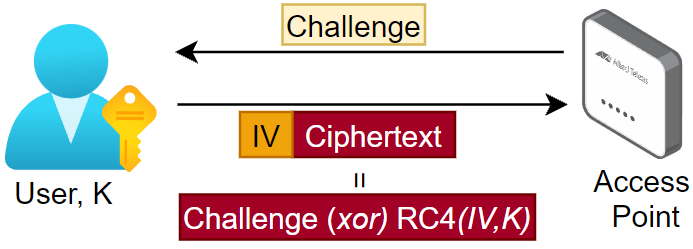
\includegraphics[width=0.8\textwidth]{image/wepchallenge.png}
    \caption{Authentication in WEP}
    \label{fig:wepchallenge}
\end{figure}
Dato che la chiave è pubblica, l'access point può verificare la conoscenza della chiave da parte dell'utente semplicemente eseguendo a sua volta lo \textit{xor}, applicando $RC4$ all'IV spedito in chiaro.\\
Le debolezze di questo sistema di auth sono le seguenti:
\begin{enumerate}
    \item Inviando la challenge in chiaro, se si dispone della relativa risposta, eseguendo \[Ciphertext\oplus{Challenge}=RC4(IV,K)\]
    si può derivare il keystream e da li è possibile produrre pacchetti firmati senza conoscere la chiave.
    \item Poiché l'initialization vector è deciso dall'implementatore, l'access point non ha modo di capire se la persona che invia la richiesta di auth è fidata. Difatti, eseguendo:
    \[
    Challenge\oplus{Challenge\oplus{RC4(IV,K)}}=RC4(IV,K)
    \]
    Esponiamo il keystream e permettendo diversi attacchi.
\end{enumerate}
Dal punto 1, capiamo che WEP finisce per implementare un KPA in quanto chiunque conosce la challenge può, costruendo un dizionario di coppie $(IV,RC4(IV,K))$, attendere che un IV si ripeta e violare il sistema.\\
Dal punto 2, si può vedere che un MITM in ascolto sul canale, può introdursi nella rete al primo IV che trova riscontro nel dizionario e da quel momento in poi restare autenticato per tutto il tempo che vuole, in quanto sarà sempre lui a decidere quale sarà l'IV da usare.\\
\begin{remark}
Una possibile soluzione, sarebbe potuta essere quella di \textbf{inviare l'IV insieme alla challenge}, in modo tale da non lasciare spazio agli utenti.
\end{remark}\pagebreak
\subsection{Errori di Integrity}
Esistono diversi algoritmi per garantire l'integrità di un pacchetto. WEP al tempo implementava $CRC-32$, un un algoritmo di error detection che può tener conto dei bit di partenza tramite bit di parità (posti alla fine del messaggio).
\begin{theorem}
$CRC-32$ è lineare nelle operazioni di $\oplus$. E' possibile modificare precisi bit del plaintext per produrre lo stesso checksum del messaggio non modificato.
\end{theorem}
\begin{proof}
La struttura del pacchetto WEP era costituita dal messaggio $M$ seguito dal codice di integrità $CRC32(M)$. Quando il messaggio viene inviato, tutti i bit vengono criptati nel seguente modo:
\[
C= M|CRC32(M)\oplus{RC4(IV, K)}
\]
Consideriamo un vettore $\delta$ di bit, lungo quanto M e contenente 1 nelle posizioni dei bit che si intende modificare nel messaggio originale.\\
Calcoliamo $CRC32(\delta)=c(\delta)$ e calcoliamo infine:
\begin{equation*}
    \begin{aligned}
    C'&=C\oplus\{\delta,c(\delta)\}\\
    &=[RC4(IV,K)\oplus{\{M,c(M)\}}]\oplus\{\delta,c(\delta)\}\\
    &=RC4(IV,K)\oplus\{M\oplus{\delta},c(M)\oplus{c(\delta)}\}\\
    &=RC4(IV,K)\oplus\{M',c(M\oplus{\delta})\}\\
    &=RC4(IV,K)\oplus\{M',c(M')\}
    \end{aligned}
\end{equation*}
Vediamo quindi che unendo al messaggio cifrato la concatenzazione $\{\delta,c(\delta)\}$ la parità misurata dall'algoritmo di controllo non risulta alterata grazie alla parità.
\end{proof}
\begin{remark}
In sintesi, il fatto che $CRC(32)$ sia lineare, risulta una debolezza per il sistema.
\end{remark}
\begin{proposition}
Un buon sistema di integrità dovrebbe garantire che:
\begin{enumerate}
    \item L'integrity checker deve essere non lineare.
    \item l'integrity checker deve esplicitamente includere una chiave, in quanto cifrature esterne non forniscono alcuna garanzia.
\end{enumerate}
\end{proposition}
\begin{remark}
Se si volesse tentare un attacco di tipo \textbf{\textit{Message Injection}} di un messaggio $M$ sarebbe ancora più facile. Una volta ottenuta una coppia valida di $(IV,RC4(IV,K))$ basta calcolare $c(M)$ e inviare $[M,c(M)]$ in xor con la la firma.
\end{remark}